\documentclass[tikz,border=12pt]{standalone}
\usepackage[T1]{fontenc}
\usepackage{mathpazo}
\usepackage{amsmath,amssymb}
\usetikzlibrary{arrows.meta, calc}

\definecolor{stblue}{HTML}{7B97AD}
\definecolor{rwgold}{HTML}{B8995E}
\definecolor{sage}{HTML}{7A9A7E}
\definecolor{dkbrown}{HTML}{3D3530}
\definecolor{wmgray}{HTML}{7B7067}
\definecolor{cream}{HTML}{F9F6F0}
\definecolor{border}{HTML}{D4C9B8}
\definecolor{terracotta}{HTML}{C47A6A}
\definecolor{lavender}{HTML}{907EA0}

\begin{document}
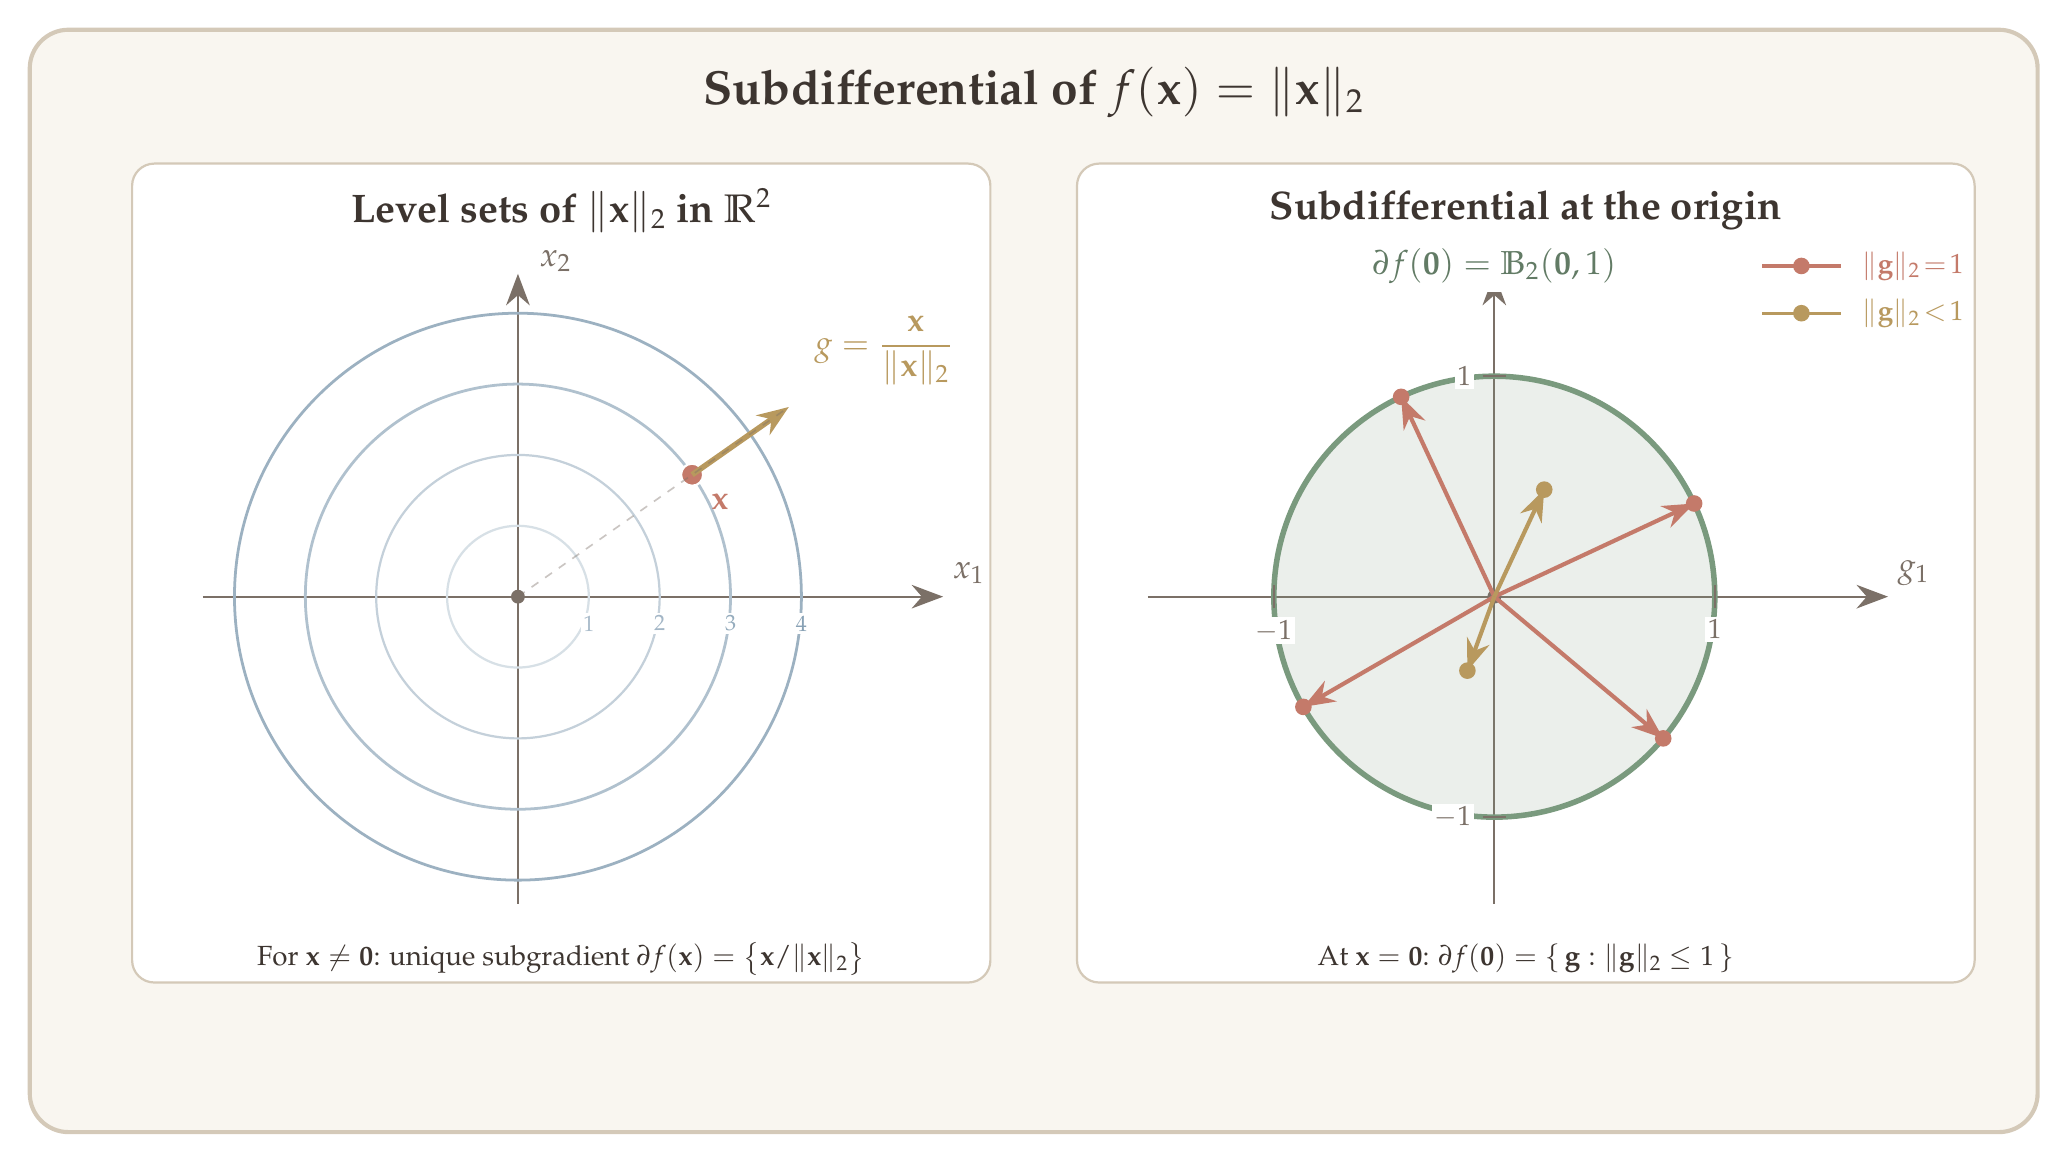
\begin{tikzpicture}[>={Stealth[length=4mm, width=3mm]}]

% Background
\fill[cream, rounded corners=14pt] (-1.0,-1.5) rectangle (24.5,12.5);
\draw[border, line width=1.5pt, rounded corners=14pt] (-1.0,-1.5) rectangle (24.5,12.5);

% Title
\node[text=dkbrown, font=\LARGE\bfseries] at (11.75,11.7)
  {Subdifferential of $f(\mathbf{x}) = \|\mathbf{x}\|_2$};

% ============================================================
% Left panel: contour plot of ||x||_2 with subgradient at x ≠ 0
% ============================================================
\fill[white, rounded corners=8pt] (0.3,0.4) rectangle (11.2,10.8);
\draw[border, line width=0.8pt, rounded corners=8pt] (0.3,0.4) rectangle (11.2,10.8);
\node[text=dkbrown, font=\Large\bfseries] at (5.75,10.2)
  {Level sets of $\|\mathbf{x}\|_2$ in $\mathbb{R}^2$};

% Left panel origin at (5.2, 5.3)
% Axes
\draw[wmgray, line width=0.8pt, ->] (1.2,5.3) -- (10.6,5.3);
\draw[wmgray, line width=0.8pt, ->] (5.2,1.4) -- (5.2,9.4);
\node[text=wmgray, font=\large, anchor=west] at (10.6,5.6) {$x_1$};
\node[text=wmgray, font=\large, anchor=south west] at (5.35,9.3) {$x_2$};

% Concentric level-set circles centered at (5.2, 5.3)
\draw[stblue!30, line width=0.8pt] (5.2,5.3) circle (0.9);
\draw[stblue!45, line width=0.8pt] (5.2,5.3) circle (1.8);
\draw[stblue!60, line width=1.0pt] (5.2,5.3) circle (2.7);
\draw[stblue!75, line width=1.0pt] (5.2,5.3) circle (3.6);

% Level set labels — along positive x1-axis, below the axis
\node[text=stblue!65, font=\footnotesize, fill=white, inner sep=1pt,
      anchor=north] at ({5.2+0.9},{5.3-0.2}) {$1$};
\node[text=stblue!70, font=\footnotesize, fill=white, inner sep=1pt,
      anchor=north] at ({5.2+1.8},{5.3-0.2}) {$2$};
\node[text=stblue!80, font=\footnotesize, fill=white, inner sep=1pt,
      anchor=north] at ({5.2+2.7},{5.3-0.2}) {$3$};
\node[text=stblue!90, font=\footnotesize, fill=white, inner sep=1pt,
      anchor=north] at ({5.2+3.6},{5.3-0.2}) {$4$};

% Origin dot
\fill[wmgray] (5.2,5.3) circle (2.5pt);

% Point x ≠ 0 (at angle 35°, on 3rd level set, radius 2.7)
\pgfmathsetmacro{\px}{5.2 + 2.7*cos(35)}
\pgfmathsetmacro{\py}{5.3 + 2.7*sin(35)}
\fill[terracotta] (\px,\py) circle (4pt);
\draw[white, line width=0.8pt] (\px,\py) circle (4pt);
\node[text=terracotta, font=\large, anchor=north west]
  at ({\px+0.12},{\py-0.12}) {$\mathbf{x}$};

% Subgradient arrow: unit vector in direction of x (from x outward)
\pgfmathsetmacro{\gx}{\px + 1.5*cos(35)}
\pgfmathsetmacro{\gy}{\py + 1.5*sin(35)}
\draw[rwgold, line width=2pt, ->] (\px,\py) -- (\gx,\gy);

% Subgradient label — to the right of arrow tip with offset
\node[text=rwgold, font=\large, anchor=south west]
  at ({\gx+0.2},{\gy+0.15})
  {$g = \dfrac{\mathbf{x}}{\|\mathbf{x}\|_2}$};

% Dashed radial line from origin through x
\draw[wmgray, line width=0.6pt, dashed, opacity=0.4]
  (5.2,5.3) -- (\gx,\gy);

% Annotation below left panel
\node[text=dkbrown, font=\normalsize, align=center] at (5.75,0.7)
  {For $\mathbf{x} \neq \mathbf{0}$: unique subgradient
   $\partial f(\mathbf{x}) = \bigl\{\mathbf{x}/\|\mathbf{x}\|_2\bigr\}$};

% ============================================================
% Right panel: subdifferential at the origin = unit ball
% ============================================================
\fill[white, rounded corners=8pt] (12.3,0.4) rectangle (23.7,10.8);
\draw[border, line width=0.8pt, rounded corners=8pt] (12.3,0.4) rectangle (23.7,10.8);
\node[text=dkbrown, font=\Large\bfseries] at (18.0,10.2)
  {Subdifferential at the origin};

% Right panel origin at (17.6, 5.3)
% Axes
\draw[wmgray, line width=0.8pt, ->] (13.2,5.3) -- (22.6,5.3);
\draw[wmgray, line width=0.8pt, ->] (17.6,1.4) -- (17.6,9.4);
\node[text=wmgray, font=\large, anchor=west] at (22.6,5.6) {$g_1$};
\node[text=wmgray, font=\large, anchor=south west] at (17.75,9.3) {$g_2$};

% Unit disk filled (radius = 2.8)
\fill[sage, opacity=0.15] (17.6,5.3) circle (2.8);
\draw[sage, line width=2pt] (17.6,5.3) circle (2.8);

% Tick marks on horizontal axis (with white fill to stay visible over circle)
\draw[wmgray, line width=0.6pt] ({17.6+2.8},{5.3-0.15}) -- ({17.6+2.8},{5.3+0.15});
\node[text=wmgray, font=\normalsize, anchor=north, fill=white, inner sep=1pt]
  at ({17.6+2.8},{5.3-0.25}) {$1$};
\draw[wmgray, line width=0.6pt] ({17.6-2.8},{5.3-0.15}) -- ({17.6-2.8},{5.3+0.15});
\node[text=wmgray, font=\normalsize, anchor=north, fill=white, inner sep=1pt]
  at ({17.6-2.8},{5.3-0.25}) {$-1$};

% Tick marks on vertical axis (with white fill)
\draw[wmgray, line width=0.6pt] ({17.6-0.15},{5.3+2.8}) -- ({17.6+0.15},{5.3+2.8});
\node[text=wmgray, font=\normalsize, anchor=east, fill=white, inner sep=1pt]
  at ({17.6-0.25},{5.3+2.8}) {$1$};
\draw[wmgray, line width=0.6pt] ({17.6-0.15},{5.3-2.8}) -- ({17.6+0.15},{5.3-2.8});
\node[text=wmgray, font=\normalsize, anchor=east, fill=white, inner sep=1pt]
  at ({17.6-0.25},{5.3-2.8}) {$-1$};

% Origin dot
\fill[wmgray] (17.6,5.3) circle (2.5pt);

% Boundary subgradient vectors (terracotta) — ||g||=1
\draw[terracotta, line width=1.5pt, ->]
  (17.6,5.3) -- ({17.6+2.8*cos(25)},{5.3+2.8*sin(25)});
\fill[terracotta] ({17.6+2.8*cos(25)},{5.3+2.8*sin(25)}) circle (3pt);

\draw[terracotta, line width=1.5pt, ->]
  (17.6,5.3) -- ({17.6+2.8*cos(115)},{5.3+2.8*sin(115)});
\fill[terracotta] ({17.6+2.8*cos(115)},{5.3+2.8*sin(115)}) circle (3pt);

\draw[terracotta, line width=1.5pt, ->]
  (17.6,5.3) -- ({17.6+2.8*cos(210)},{5.3+2.8*sin(210)});
\fill[terracotta] ({17.6+2.8*cos(210)},{5.3+2.8*sin(210)}) circle (3pt);

\draw[terracotta, line width=1.5pt, ->]
  (17.6,5.3) -- ({17.6+2.8*cos(320)},{5.3+2.8*sin(320)});
\fill[terracotta] ({17.6+2.8*cos(320)},{5.3+2.8*sin(320)}) circle (3pt);

% Interior subgradient vectors (rwgold) — ||g||<1
\draw[rwgold, line width=1.5pt, ->]
  (17.6,5.3) -- ({17.6+1.5*cos(65)},{5.3+1.5*sin(65)});
\fill[rwgold] ({17.6+1.5*cos(65)},{5.3+1.5*sin(65)}) circle (3pt);

\draw[rwgold, line width=1.5pt, ->]
  (17.6,5.3) -- ({17.6+1.0*cos(250)},{5.3+1.0*sin(250)});
\fill[rwgold] ({17.6+1.0*cos(250)},{5.3+1.0*sin(250)}) circle (3pt);

% Subdifferential label — centered above circle, with white fill to avoid axis overlap
\node[text=sage!80!black, font=\large\bfseries, fill=white, inner sep=3pt]
  at (17.6,9.5) {$\partial f(\mathbf{0}) = \mathbb{B}_2(\mathbf{0},1)$};

% Legend: boundary vs interior (upper right corner of panel)
\fill[terracotta] (21.5,9.5) circle (3pt);
\draw[terracotta, line width=1.2pt] (21.0,9.5) -- (22.0,9.5);
\node[text=terracotta, font=\normalsize, anchor=west] at (22.15,9.5)
  {$\|\mathbf{g}\|_2\!=\!1$};

\fill[rwgold] (21.5,8.9) circle (3pt);
\draw[rwgold, line width=1.2pt] (21.0,8.9) -- (22.0,8.9);
\node[text=rwgold, font=\normalsize, anchor=west] at (22.15,8.9)
  {$\|\mathbf{g}\|_2\!<\!1$};

% Annotation below right panel
\node[text=dkbrown, font=\normalsize, align=center] at (18.0,0.7)
  {At $\mathbf{x} = \mathbf{0}$: $\partial f(\mathbf{0})
   = \{\,\mathbf{g} : \|\mathbf{g}\|_2 \leq 1\,\}$};

\end{tikzpicture}
\end{document}
